\section{Introduction}

\par Bytes of data, or short sequences of 1s and 0s, are exchanged between
computer systems each day on public channels.
Because gentlemen do read each other's mail, it is necessary to secure the
communication of private data sent over public channels. The solution to this
problem is solved by {\em cryptography}, the designing of systems to secure
data exchanges over public channels.

\par The following example is the same basic communication scenario presented
by Trappe in \cite{bk:tw06}.
Let there be two parties, Alice and Bob, who wish to communicate with one another.
A third party, Eve, is a potential eavesdropper. Alice wants to send a message,
known as the {\em plaintext}, to Bob. To accomplish this without Eve knowing
what the message is before it is received by Bob, Alice must {\em encrypt} her message
by some prearranged method, usually involving an {\em encryption key}, to generate
a related message called {\em ciphertext}. The idea is that the sent ciphertext,
even if it is intercepted by Eve, will be too difficult to interpret and will conceal the
plaintext message. Upon receipt of the ciphertext, Bob will {\em decrypt} the message,
usually involving a {\em decryption key}, similar to the encryption of the message,
and obtain the plaintext message. A visual of this scenario is presented in \cite{fig:basic-scenario}.

\begin{figure}[h!]\label{fig:basic-scenario}
	\centering
		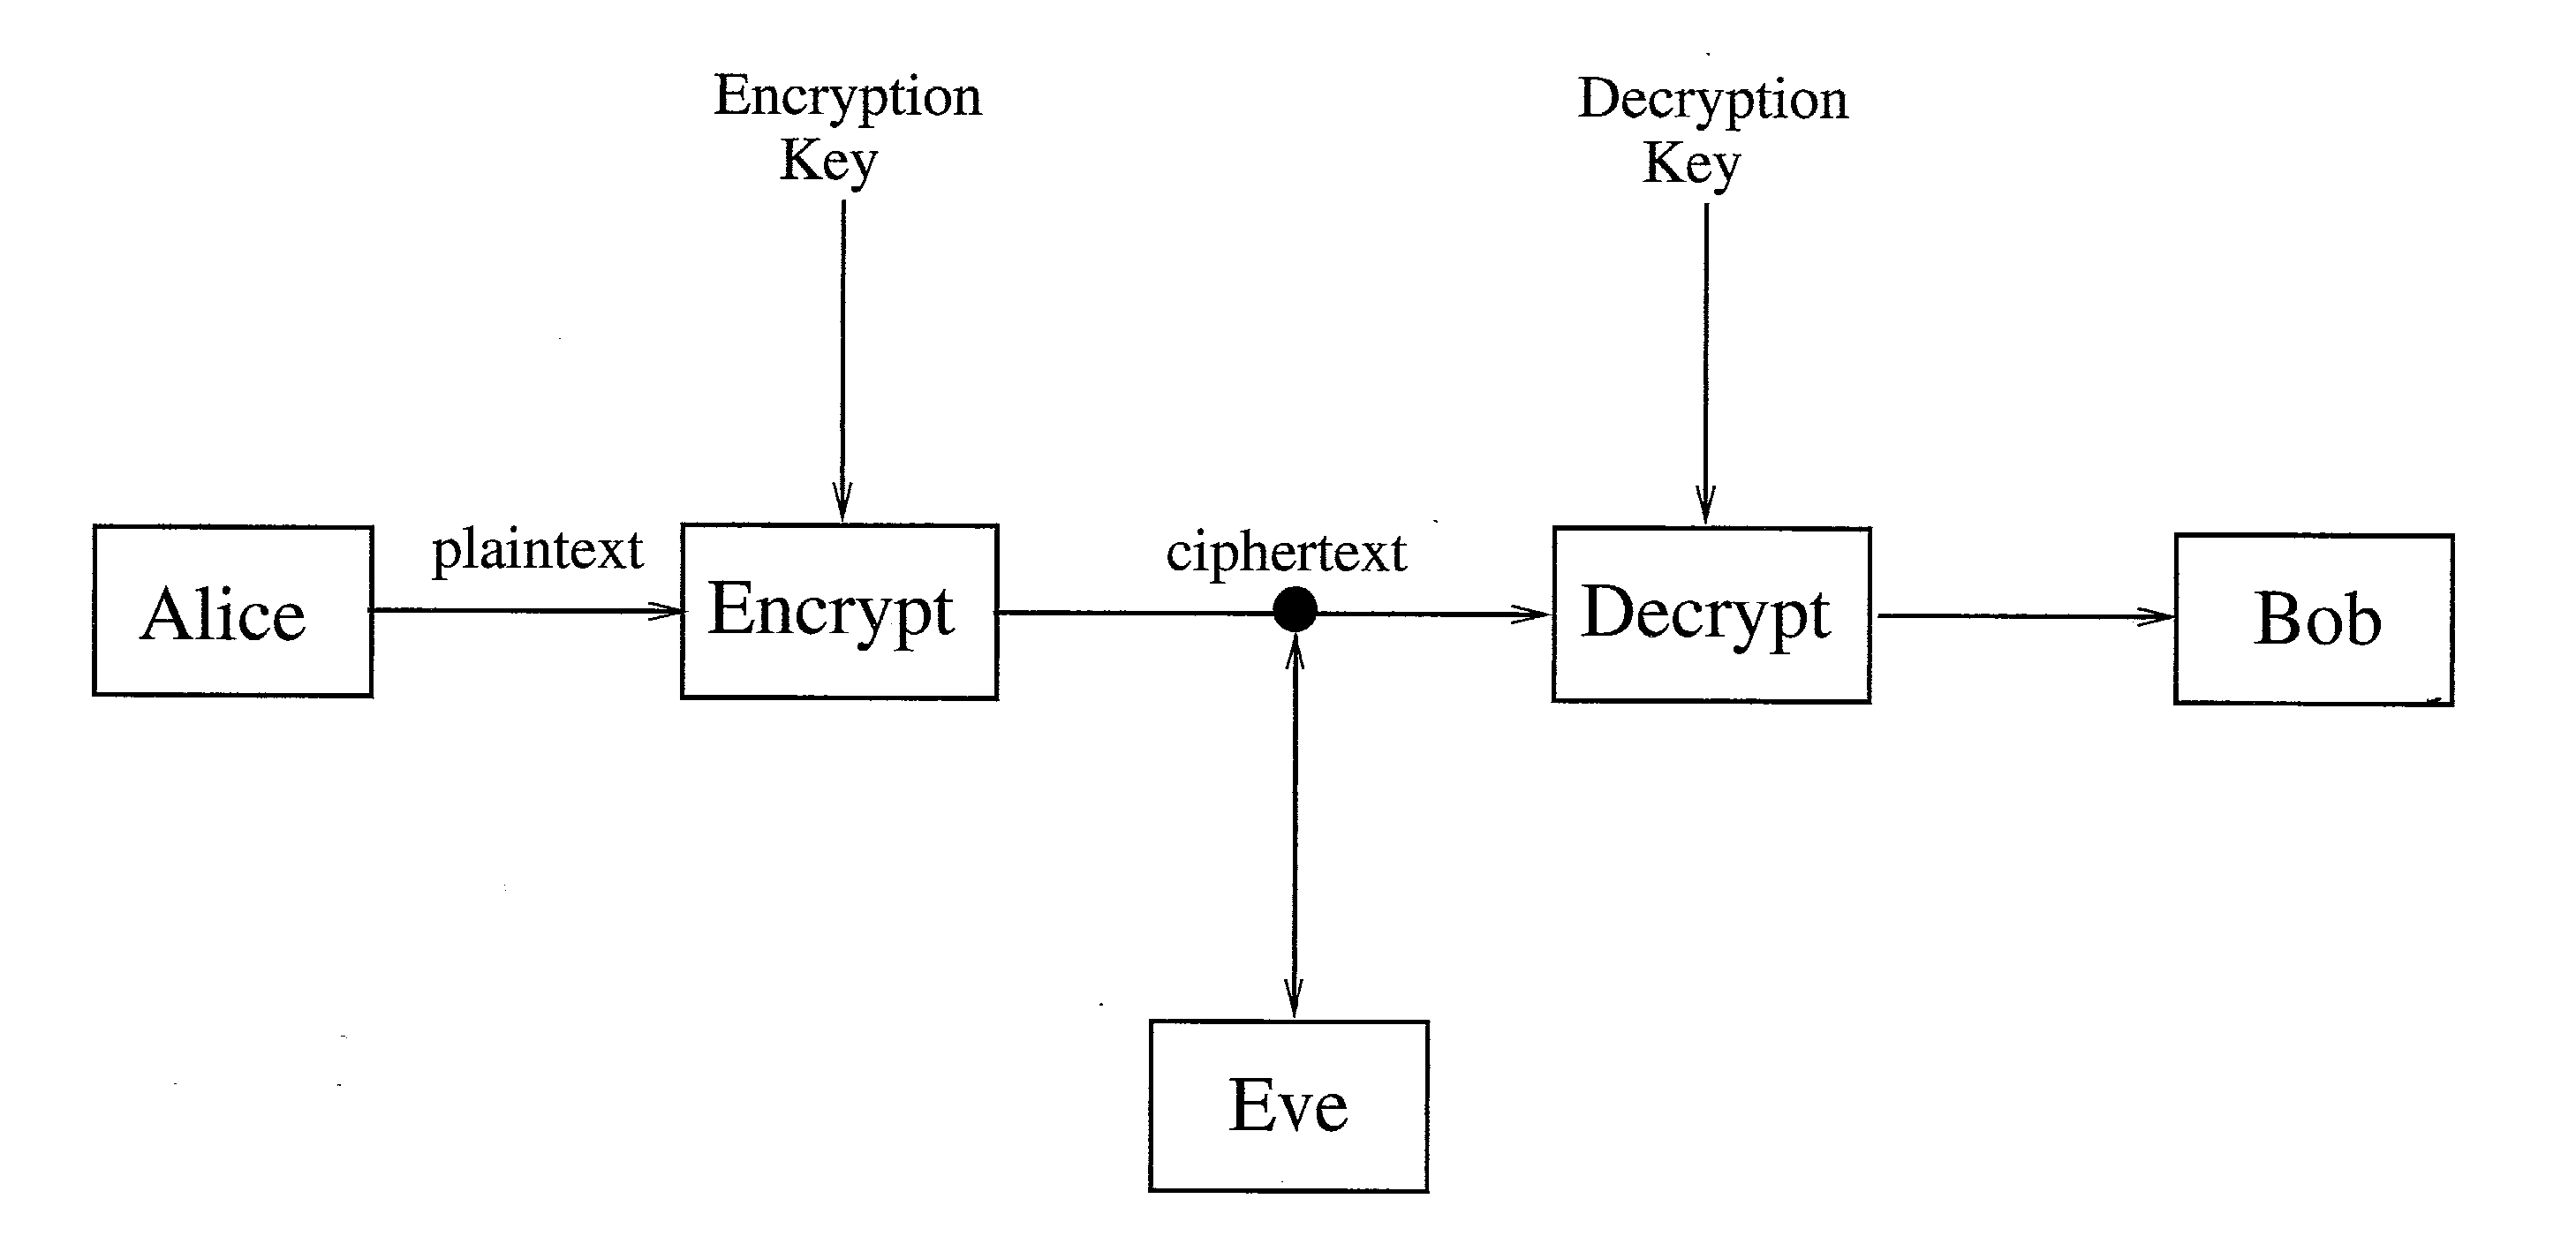
\includegraphics[width=120mm]{figs/basic-scenario.png}
		\caption{The Basic Comunication Scenario for Cryptography \cite{bk:tw06}}
\end{figure}

\par This scenario is the standard example found in many different introductory
cryptography references. Cryptographers have created numerous encryption and decryption
schemes, or {\em cryptosystems}, to secure the messages sent between Alice and Bob.
Many of these systems have been broken because of the amount of work that goes into
the study of breaking cryptosystems, called {\em cryptanalysis}. A constant battle
exists between the designers and breakers of cryptosystems, strengthening designs and attacks every day.
In fact, designing a strong cryptosystem typically requires knowledge of cryptography and cryptanalysis.

\par Before diving into the topic of this paper, there is an important assumption that must
be presented. When designing a cryptosystem, every cryptographer assumes {\em Kerckhoffs' principle} \cite{bk:tw06}:
``In assessing the security of a cryptosystem, one should always assume the enemy knows the method
being used.'' The security of a cryptosystem
cannot be based on the concealment of the encryption and decryption algorithms. In practice,
the enemy can obtain the algorithms in many ways, including the defection or capture
of people. The security must be based on the key and not the algorithm. 

\par Imagine that Alice's message to Bob is a sequence of 1s and 0s, as it would be
in the real world. Consider a cryptosystem which encrypts each bit in the sequence
separately. This would be done by what is called a {\em stream cipher}, which, according to Rueppel,
divides bit sequence into individual bits and enciphers each bit with a time-varying
function whose time-dependency is governed by the internal state of the stream cipher \cite{rueppel_book}.
The stream cipher can also be thought of in terms of a {\em keystream} which is a
sequence of 1s and 0s the same length of the message that is added to the message
using addition in $\gftwo$ (also known as XOR). If the keystream was perfectly random,
then the cryptosystem would be unbreakable, or {\em perfectly secret}, as
discovered by Claude Shannon in his famous paper ``Communication Theory of Secrecy Systems,''
written in 1945 and published in 1949. This cryptosystem is known as the {\em one-time pad}.
Though it is perfectly secret, it can be difficult to implement because of the inability
to produce perfectly random keystreams. Constructing a method to produce perfectly random
sequences is a contradiction in itself.% If there is a method to produce the sequence,
%then it cannot be perfectly random.

\par Though it is impossible to create perfectly random sequences, it is possible to get close.
This type of sequence is called a {\em pseudorandom sequence}. These sequences have extremely
long periods but are statistically indistinguishable from random sequences. This paper will discuss
the construction of pseudorandom sequences using a particular finite state machine
called the {\em feedback with carry shift register}. It will also investigate the possibility of
incorporating {\em bent functions}, or perfectly non-linear functions, into the construction of
psuedorandom sequences in an attempt to resist synthesizing algorithms. 

%\par The paper will follow this basic outline. Important properties of the $N$-adic integers
%will be established and examples of different various kinds of $N$-adic integers will be given. 
%Then, the finite-state machine will be introduced, followed by the definition of the feedback
%with carry shift register. Finally, the boolean functions are defined and described and various
%theorems and conjectures will be presented on bent functions.
